\chapter{Developement version of pixel ordering}
\section{Image data}
Nominal size of CCD sensor is 4096x4096 pixels. Each pixel is sampled with 18-bit resolution and consists of two samples: one of video level and another of black level. This gives in total 4096x4096x2x2 = 64MB of data. Due to high SNR requirements each pixel has to be oversampled. Two agreed oversampling factors are 4x and 16x. Taking into account oversampling, final frame sizes are respectively 256MB and 1024MB. \\
Image data is contained in one continuous memory block but due to CCD readout and oversampling method, order of image pixels in memory is different than physical one in CCD matrix. CCD matrix is divided into four identical groups of pixels which have independent readout channels as shown on figure \ref{fig:readout}. \\
Due to order of ADC triggering final image data layout is different. Image data ordering in memory (for 4x oversampling mode) is presented on figure \ref{fig:oversample4}.

%\begin{figure}[H]
%\centering
%\includesvg[clean, pretex=\relscale{0.7}, width=\textwidth, svgpath = pict_ipc/]{image_data_format}
%\caption{Image data format for 4x oversampling}
%\label{fig:oversample4}
%\end{figure}

\begin{figure}[H]
\centering
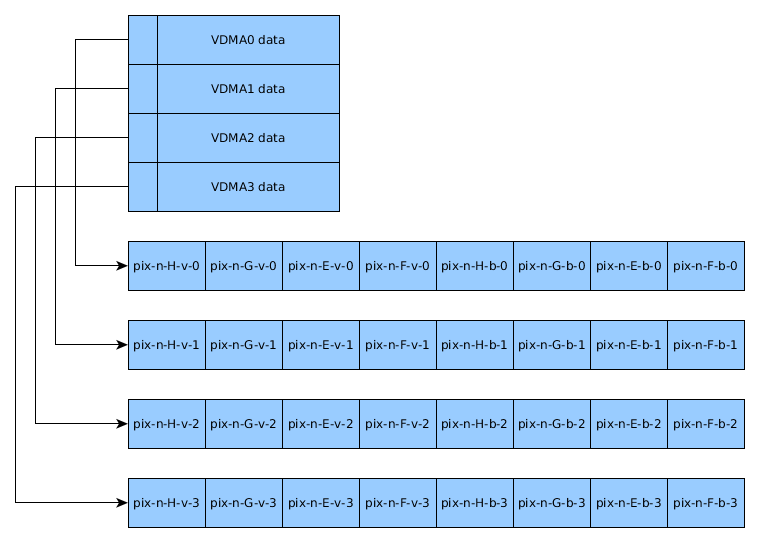
\includegraphics[width=\textwidth]{pict_ipc/image_data_format.png}
\caption{Image data format for 4x oversampling}
\label{fig:oversample4}
\end{figure}

\emph{pix-n-H-v-0} means: n-th pixel from section H video level sample 0. Similarly \emph{pix-n-E-b-2} means: n-th pixel from section E black level sample 2.

\section{Sensors list}

\begin{table}
\footnotesize
\begin{tabular}{ | l | l | l | l | l | l | l | l | l | }
\hline
	Board & Parameter & Sensor & Resolution & Accuracy & Range & Ext. Range & \begin{tabular}{@{}c@{}} Max Read \\ Freq. [Hz] \end{tabular} & Qty \\ \hline
	Comm. & Humidity & STH25 & 0,04 \%RH & +/- 1,8 \%RH & 10 – 90 \%RH & 0-100 \%RH & 0.125 & 1 \\ \hline
	 & Temperature &  & 0,04 \degree C & +/- 0,2 \degree C & 0-60 \degree C & -40-120 \degree C & 0,2 – 0,033 & 1 \\ \hline
	 & Temperature & MAX6639 & 0,125 \degree C & +/- 1\degree C & 0 – 125 \degree C & - & 8(1) & 1 \\ \hline
	Main & Humidity & HDC1000 & 0,006\%RH & +/- 3 \%RH & 10 – 80 \%RH & 0-100 \%RH & 6.6E-2 & 1 \\ \hline
	 & Temperature &  & 0,01 \degree C & +/- 0.2 \degree C & -40-125 \degree C & - & - & 1 \\ \hline
	 & Acceleration & ADXL343 & 0,004g & +/- 1\% & \begin{tabular}{@{}c@{}}+/-16g,+/-8g \\ +/-4g/+/-2g\end{tabular} & - & 0.1 – 3200 & 1 \\ \hline
	 & Temperature & ADS1248 & 5,96u \degree C & +/- 1\degree C & +/- 50\degree C & - & 5-2000 & 3 \\ \hline
	 & Coolant flow & MAX6639 & - & +/- 3\degree C & 2000-16000RPM & - & - & 1 \\ \hline
	 & T. alarm (set) & LM75 & 0,3515625\degree C & +/- 2,\degree C & -55 – 125 \degree C & - & 0.33 & 1 \\ \hline
	CCD & Humidity & HDC1000 & 0,006\%RH & +/- 3 \%RH & 10 – 80 \%RH & 0-100 \%RH & 6.6E-2 & 1 \\ \hline
	 & Temperature &  & 0,01 \degree C & +/- 0.2 \degree C & -40-125 \degree C & - & - & 1 \\ \hline
\end{tabular}
\end{table}
